\documentclass[letterpaper]{article}
\usepackage{listings}
\usepackage{booktabs}
\usepackage{array}
\usepackage{multirow}
\usepackage{amsmath,amssymb}
\usepackage{hhline}
\usepackage{authblk}
\usepackage[T1]{fontenc}
\usepackage{lipsum}
\usepackage{float}
\usepackage{graphicx}
\usepackage[export]{adjustbox}
\usepackage{caption}
\usepackage{subcaption}
\usepackage[final]{pdfpages}
\usepackage{wrapfig}
\renewcommand{\baselinestretch}{2}

\usepackage[letterpaper, margin=1in]{geometry}

\begin{document}
	
	\begin{titlepage}
		\begin{center}
			\vspace*{1cm}
			
			\Huge
			\textbf{North Shore Rail Extension}
			
			\vspace{2.5cm}
			\textbf{User Manual \\}
			\vspace{2.5cm}
			\textbf{Low-comotivation}
			\vspace{2.5cm}
			
		\end{center}
		
		\begin{flushright}        
			\Large
		\end{flushright}        
		
		\vfill
		\begin{center}        
			
			\vspace{0.8cm}        
			
			\Large
			COE1186 - Software Engineering\\
			Instructor: Joseph A Profeta III, Ph.D.\\
			Spring 2017
			
		\end{center}
	\end{titlepage}

\cleardoublepage
\setcounter{tocdepth}{1}
\tableofcontents

\begin{center}
	\Large
	\title{CTC/Office User Manual}
	\author {Written by: Christen Reinbeck}
	\date{}	
\end{center}

\maketitle

\section{CTC}

\subsection{UI Layout}

\begin{figure}[h!]
	\centering
	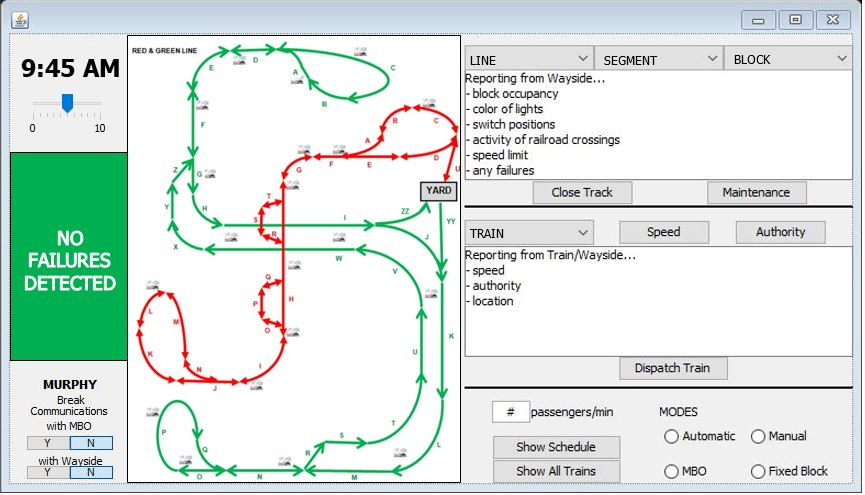
\includegraphics[width=16cm]{CTC_gui}
	\caption{Graphical User Interface for the CTC}
\end{figure}

\subsection{UI Buttons and Actions}

\subsubsection{Time/Fast-Forward Capability}
\begin{itemize}
	\item Slider - used to control speed of time passing, either regular speed or 10x speed.
	\item Clock - displays time in whatever speed is selected.
\end{itemize}

\subsubsection{Failure Detection Sidebar}
\begin{itemize}
	\item Sidebar color change block - sidebar will display in one of two ways:
	\begin{itemize}
		\item Green: no failures detected
		\item Red: Failure detected as well as in which line/segment/block
	\end{itemize}
\end{itemize}

\subsubsection{Murphy}
\begin{itemize}
	\item Slider buttons - ability to activate communication breaks between either MBO or Wayside controller for testing purposes.
\end{itemize}

\subsubsection{Line Map}
\begin{itemize}
	\item Displays all sections and lines of the map/system you are currently working on.
\end{itemize}

\subsubsection{Block Controls}
\begin{itemize}
	\item Dropdowns - used to select appropriate line/segment/block that you wish to use.
	\item Text display - displays information as pulled from wayside controller, such as block occupancy, switch status, light color and status, activity of railroad crossings, and block failures.
	\item Close track button - propagates a popup window that restates which block of track you wish to close with either the option to close track or cancel.
	\item Send maintenance button - propagates a popup window that restates which block of track you wish to send maintenance to, with either the option to send or cancel.
\end{itemize}

\subsubsection{Train Controls}
\begin{itemize}
	\item Dropdown - used to select a specific train.
	\item Speed and Authority Buttons - propagates popup windows where you can set speed or authority for a given train.
	\item Text display - displays the current speed and authority of the selected train, and updates should the user change the speed and authority at a given time.
	\item Dispatch train button - propagates a popup window which allows you to dispatch a train from the yard, selecting line, station to go to, speed and authority.
\end{itemize}

\subsubsection{Miscellaneous Controls/Info}
\begin{itemize}
	\item Throughput display - displays number of passengers/hour of the system as a whole.
	\item Show schedule button - propagates a popup window of train schedules from the MBO/Scheduler.
	\item Show all trains button - propagates a popup window of all trains currently dispatched as well as their current GPS location, line, segment, block.
	\item Mode Options for Schedule via radio buttons:
	\begin{itemize}
		\item Automatic - this mode gives the dispatcher two options
		\begin{itemize}
			\item MBO - gets a schedule from the MBO/Scheduler that is most optimized with more trains running.
			\item Fixed Block - also gets a schedule from the MBO/Scheduler but only allows one train/block at any given time.
		\end{itemize}
		\item Manual - dispatcher manually dispatches trains using the aforementioned button.
	\end{itemize}
\end{itemize}

\newpage

\begin{center}
\Large
\title{Wayside Controller User Manual \\}
\author{Written by: Max Reno}
\date{}	
\end{center}


\maketitle

\section{Wayside Controller}

\subsection{UI Layout}

\begin{figure}[h!]
	\center
	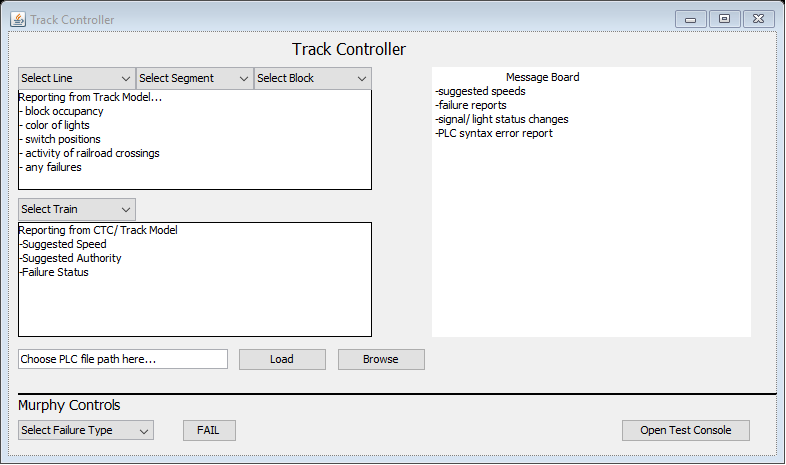
\includegraphics[width=16cm]{trackcontroller_gui}
	\caption{Graphical User Interface for the track controller.}
\end{figure}


\subsection{UI Buttons and Actions}

\subsubsection{Block Selection}
\begin{itemize}
	\item Series of Dropdowns - used to select appropiate line/segment/block
	\item Text Display - displays information such as block occupancy, switch status, light color and status, activity of railroad crossings and any failures that it may report to the CTC.
\end{itemize}
\subsubsection{Train Selection}
\begin{itemize}
	\item Text Display - reports on the suggested speed and authority as received from the CTC as well as any failures which would need to be reported back the CTC/track model.
\end{itemize}
\subsubsection{File Browser/Loader}
\begin{itemize}
	\item Text Field - can input file path here directly or use the browse option as follows.
	\item Load Button - Load button - once file is chosen, pressing load will load the given PLC file and run it accordingly.
	\item Browse button - this will propagate a pop up window which will allow the user to browse through their computer to find the appropriate file that they wish to load.
\end{itemize}
\subsubsection{Message Board}
\begin{itemize}
	\item Text display - this field will display any info that doesn't apply to the two other fields such as: debugging PLC or changing failures statuses.
\end{itemize}
\subsubsection{Murphy}
\begin{itemize}
	\item Dropdown - select the type of failure that the user wishes to instantiate.
	\item Fail button - instantiates the given type of failure.
	\item Open Test Console button - pushing this button opens a pop up window of the testing console as follows.
\end{itemize}


\subsection{UI Testing Layout}

\begin{figure}
	\center
	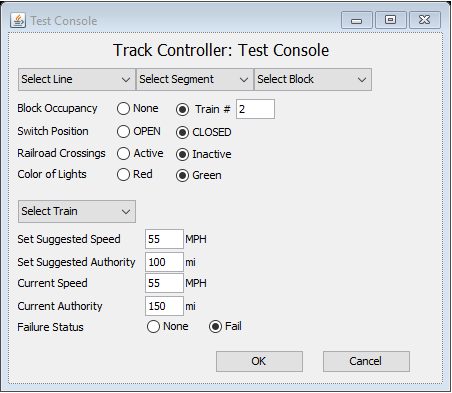
\includegraphics[width=10cm]{trackcontrollertestconsole_gui}
	\caption{Graphical user Interface for the test console of the wayside controller.}
\end{figure}


\subsection{UI Buttons and Actions}

\subsubsection{Block Selection}
\begin{itemize}
	\item Series of Dropdowns - used to select appropriate line/segment/block.
\end{itemize}

\subsubsection{Block Testing Situations}
\begin{itemize}
	\item Series of Radio Buttons -
	\begin{itemize}
		\item Block Occupancy - either clears the block of all trains or adds a given train into this block in order to report on it.
		\item Switch Position - closed will keep it in the same position, while open will change it.
		\item Railroad Crossings - triggers them to be on or off should a given block have them.
		\item Color of lights - triggers the lights to either color in order to report on it.
	\end{itemize}
\end{itemize}

\subsubsection{Train Testing Situations}
\begin{itemize}
	\item Series of Text Inputs - allows user to give inputs as if the track/CTC didn't exist in order to test it on its own.
\end{itemize}
\subsubsection{Ok/Cancel Buttons - passes the information chosen here onto the original UI to show testing.}

\newpage

\begin{center}
	\Large
	\title{Track Model User Manual \\}
	\author{Written by: Michael Ghaben}
	\date{}	
\end{center}

\maketitle


\section{Track Model}

\subsection{UI Layout}
\begin{figure}[h]
	\centering
	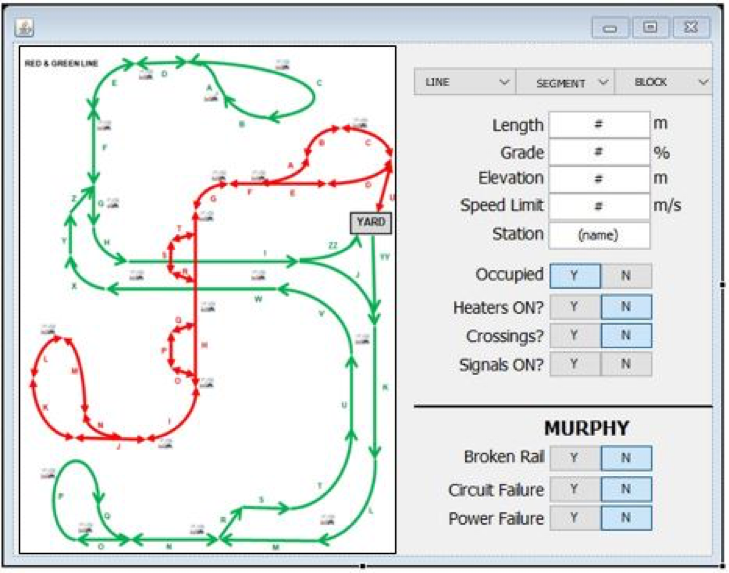
\includegraphics{trackUI}
	\caption{The current Track UI layout}
\end{figure}


\subsection{UI Buttons and Actions}

	\subsubsection{Line, Section, and Block Selection}
		\begin{itemize}
			\item Line Selection - The user may select the line to view from the "line" dropdown list of lines
			\item Section - The user may select the section to view from the "section" dropdown menu
			\item Block - The user may select the block from the block dropdown menu
		\end{itemize}
		After selecting the Line / Section / Block, the user may view the pertinent information on the panels of the screen.
	\subsubsection{Static Information}
	The user may view the static information about the track on the righthand panel. This information will be loaded into the program via an excel file at initialization. The following information is displayed:
		\begin{itemize}
			\item Length - The length of the selected block (feet)
			\item Incline / Grade - The grade of the selected block (percent)
			\item Elevation - The elevation of the selected block (feet)
			\item Speed Limit - The speed limit of the selected block (miles per hour)
			\item Station - If a station is on this block, a station name will be given. If there is no station on the block, this field will be empty
		\end{itemize}
		The values will be provided in imperial units. Furthermore, the track direction and infrastructure (such as underground) will be reflected in the graphical display on the left. Track direction will be marked with the arrows as shown, and infrastructure will be marked via a drawing scheme. Switches will be marked graphically with an "open" or "closed" on the map between the sections which are connected.

\subsection{Dynamic Information}
		Additionally, the following dynamic information will be provided based upon the runtime environment of the train system:
		\begin{itemize}
			\item Occupied - Is the selected block of the track occupied
			\item Heaters - If the selected block has heaters, are they on?
			\item Crossings - Are railway crossings down? ("Yes" implies the railway crossings are down)
			\item Signals ON - Are the train light signals currently on?
		\end{itemize}
		The railway crossings terminology may be changed as to make the information presented clearer.

\subsection{User Control}
In this module, no control of the tracks state from the external user interface is provided. This is a reflection of the underlying philosophy that the track model itself should be "dropped out" and replaced by a physical track when the end user (the train company). In this case, the track models primary duties -- loading passengers onto the track and turning the heaters on and off -- will be handled automatically, with the ability to programmatically control the variables.

\newpage

\begin{center}
	\Large
	\title{Train Model User Manual \\}
	\author{Written by: Demetri Khoury}
	\date{}	
\end{center}

\maketitle


\section{Train Model}

\subsection{UI Layout}

\begin{figure} [h!]
	\center
	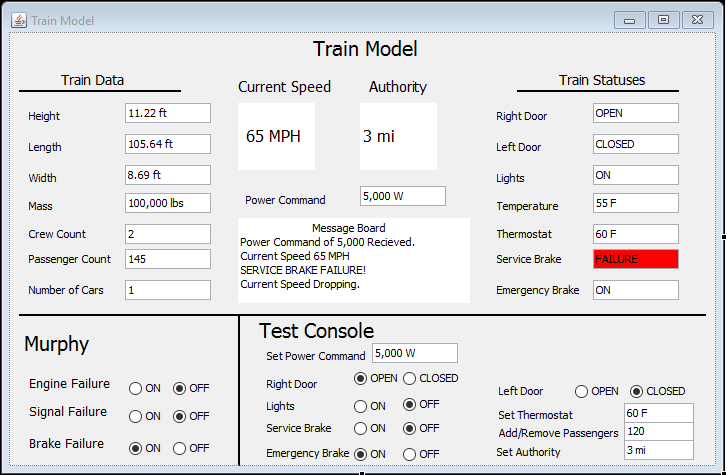
\includegraphics[width=16cm]{trainmodel_gui}
	\caption{Graphical User Interface for the train model}
\end{figure}


\subsection{UI Buttons and actions}

\subsubsection{Train Data}
\begin{itemize}
	\item Height:  Displays the Height of the train being observed. The height is a constant value obtained from the provided train data sheet.
	\item Length: This value will be displayed to provide the length of the train observed. This value will update as cars are added and removed from the train. From the train data sheet, it was observed that each car was about 106 feet long.
	\item Width:  Displays the width of the train being observed. The width is a constant value obtained from the provided train data sheet.
	\item Mass: This value displays the mass of the train. This will update based on the number of cars attached and number of passengers onboard.
	\item Crew Count: This field displays the number of crew members currently operating the train. This will update based worker schedule as crew members enter and exit.
	\item Passenger Count: This displays the total number of passengers currently on the train. This value will update as passengers embark and disembark.
	\item Number of Cars: This field displays the number of cars currently attached to the train. This will update as cars are added or removed.
\end{itemize}

\subsubsection{Center Console}
\begin{itemize}
	\item Current Speed:  Displays the current speed of the train. This will be tracked and the value will update periodically as the system runs.
	\item Current Authority:  This value displays the current Authority of the train. This will update accordingly as a new authority is passed to the train from the track.
	\item Power command: This will display the current power command issued to the train model from the train controller. This power will determine the new speed of the train.
	\item Message Board: This section of the console will display event and failure logs of the system periodically as they occur. Notifications such as incoming power commands, current speed and failure statuses will be displayed here
\end{itemize}

\subsubsection{Train Statuses}
\begin{itemize}
	\item Right Door:  Displays the status of the right doors of the train. This will either be shown as "OPEN", "CLOSED" or "FAILURE".
	\item Left Door:  Displays the status of the left doors of the train. This will either be shown as "OPEN", "CLOSED" or "FAILURE".
	\item Lights:  Displays the status of the interior lights of the train. This will either be shown as "ON", "OFF" or "FAILURE".
	\item Temperature: This will display the current temperature inside the train. This will update periodically based on the temperature changes onboard.
	\item Thermostat: This will display the current thermostat settings onboard the train. This will update periodically based on the value set in the train controller.
	\item Service Brake:  Displays the status of the Service brake of the train. This will either be shown as "ON", "OFF" or "FAILURE".
	\item Emergency Brake:  Displays the status of the Service brake of the train. This will either be shown as "ON", "OFF" or "FAILURE".
\end{itemize}
	\subsubsection{Murphy Controls}
	\begin{itemize}
		\item Engine Failure: This radio button allows for the user to toggle an engine failure onboard the train.
		\item Signal Failure: This radio button allows for the user to toggle a signal failure onboard the train.
		\item Brake Failure: This radio button allows for the user to toggle a failure in the trains service brakes.
	\end{itemize}

	\subsubsection{Test Console}
	\begin{itemize}
		\item Test Console: This console will allow for simulation of the train model without external input from the train controller. This will allow for the user to toggle various inputs that would otherwise be received from the train controller. Changes from these inputs will be displayed in the upper half of the UI.
		\item Set Power Command: This text field will allow the tester to input a new power command for the train model.
		\item Right Door: This radio button will toggle the right doors between open and closed
		\item Left Door: This radio button will toggle the left doors between open and closed
		\item Lights: This radio button will toggle the interior lights between on and off
		\item Service Brake: This radio button will toggle the service brakes on the train from on and off
		\item Emergency Brake: This radio button will toggle the emergency brakes on the train between on and off
		\item Set thermostat: This text field will allow the test user to input a new thermostat setting for the train.
		\item Add/Remove Passengers: This text field will allow for the test user to input the number of passengers embarking and disembarking at each station. A positive value will add to the current passenger count and a negative value will subtract from the current passenger count
		\item	Set Authority: This text field will allow the test user to set a new authority for the train.
	\end{itemize}

\newpage

\begin{center}
	\Large
	\title{Train Controller User Manual \\}
	\author{Written by: Andrew Lendacky}
	\date{}	
\end{center}

\maketitle


\section{Train Controller}

\subsection{UI Layout}

\begin{figure}[h!]
	\center
	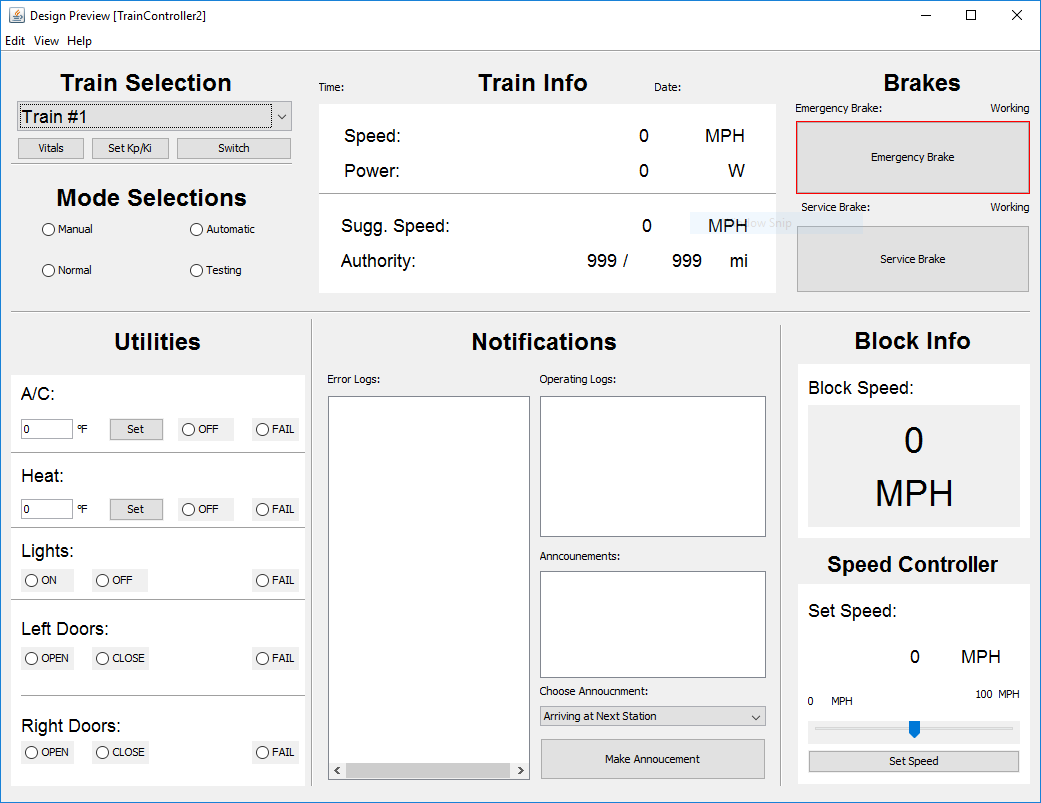
\includegraphics[width=16cm]{traincontroller_gui.PNG}
	\caption{Graphical User Interface for the train controller.}
\end{figure}

\begin{figure}[h!]
	\center
	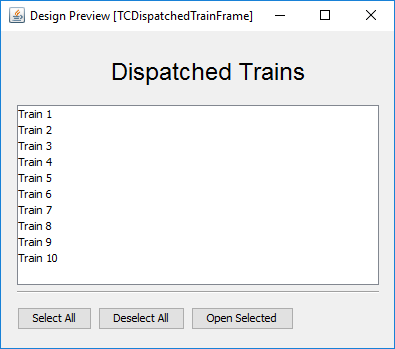
\includegraphics[width=10cm]{traincontroller_dispatchedtrains.PNG}
	\caption{User Interface for the dispatched trains.}
\end{figure}

\begin{figure}[h!]
	\center
	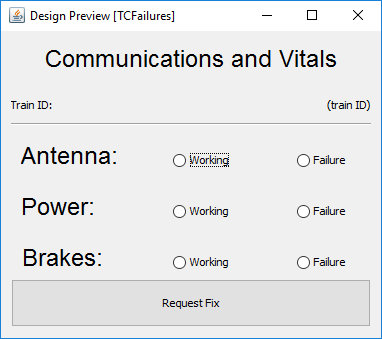
\includegraphics[width=10cm]{traincontroller_failurepanel.PNG}
	\caption{User interface for monitoring the failures of a train.}
\end{figure}

\begin{figure}[h!]
	\center
	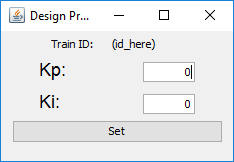
\includegraphics[width=10cm]{traincontroller_engineerpanel.PNG}
	\caption{User Interface for setting $K_p$ and $K_i$.}
\end{figure}

\subsection{UI Buttons and Actions}

	\subsubsection{Train Selection}
		\begin{itemize}
			\item Train Selection Dropdown - Clicking on the dropdown will allow the user to select a dispatched train.
			\item Switch - Clicking on this button will change the controls of this Train Controller to that of the selected train. 
			\item Vitals - Clicking on this button opens the Failures window (Figure 3) to monitor the status of the 3 failures that can occur on the train. If any failures exist, the button will be red.
			\item Set $K_p$/$K_i$ - Allows the user to control the power constants, $K_p$ and $K_i$. Clicking on this opens up Engineering Panel (Figure 4).
		\end{itemize}
	\subsubsection{Brake Controls}
	The operating status of both the emergency and service brakes can be seen above their respective button.
		\begin{itemize}
			\item Emergency Brake Button - Clicking on this button will open a window to confirm if you want to initiate the emergency brakes of the selected train. Clicking 'confirm' will apply the emergency brakes.
			\item Service Brake Button -  Clicking on this button will initiate the service brakes of the selected train.
		\end{itemize}
	
	\subsubsection{Speed Controller}
		\begin{itemize}
			\item Speed Slider - This slider controls setting the speed of the selected train. The max value of this slider is the max speed the train is allowed to go. In manual mode the max speed is determined by the block speed, and in automatic mode, the max speed is the suggested speed determined by the CTC.
			\item Set Speed Button - Clicking this button sends the selected speed to the train. 
		\end{itemize}
	\subsubsection{Block Information}
		\begin{itemize}
			\item Block Speed - This label displays the max speed of the block the selected train is in (miles per hour).  
		\end{itemize}
	\subsubsection{Train Information}
		\begin{itemize}
			\item Speed - Displays the speed the selected train is going (miles per hour). 
			\item Power - Displays the power the selected train is producing (watts). 
			\item Suggested Speed - Displays the speed that was suggested by the dispatcher (miles per hour). 
			\item Authority - Displays the authority that was set by the dispatcher and how much distance has elapsed (in miles).
		\end{itemize}
	\subsubsection{Mode Selections}
		\begin{itemize}
			\item Auto and Manual - Lets the user switch between Manual and Automatic mode. 
				\begin {itemize}
					\item Manual - The user controls the states of the selected train's Utilities (ON, OFF, OPEN, CLOSED, FAIL), controls the speed and initiates both brakes, as well as request repairs for any failures. 
					\item Automatic - The user cannot control the states of the selected train's Utilities (ON, OFF, OPEN, CLOSED, FAIL), the speed, repair requests, and the service brake. The user can only control the emergency brakes.
				\end{itemize}
			\item Normal and Testing - Lets the user switch between Normal and Testing mode. 
				\begin {itemize}
					\item Normal - The train controller operates cooperatively with all modules in the system. 
					\item Testing - Opens a window that allows the user to operate the Train Controller without the other necessary modules. 
				\end{itemize}
		\end{itemize}
	\subsubsection{Notifcations}
		\begin{itemize}
			\item Error Logs - Displays any errors or failures that the selected train has or had and at what time.
			\item Operating Logs - Displays operating logs about selected train.
			\item Announcements - Displays any previously made announcements to the screen and at what time. 
			\item Choose Announcement Dropdown - If in manual mode, lets the user pick from a list of available announcements to make. 
			\item Make Announcement Button - Transmits the selected announcement from the announcement dropdown through the train's speaker system. 
		\end{itemize}
	\subsubsection{Utilities}
	Manual Mode: The driver can change the state of these utilities as well as set the desired temperature of the air conditioning and heating unit. If any of the utilities are in the FAIL state, they must be fixed before the driver can change their state. Attempting to change the state while in FAIL will result in a error window. To request a fix, go to View > Failures from the menu bar or click 'Vitals' under the train selection dropdown.
	\newline
	Automatic Mode: The user cannot control the states of these buttons, and are set according to the instruments (thermostat, light sensor, etc..) on the train. The status of these buttons will be selected based on the states of utilities on the selected train.
		\begin{itemize}
			\item Air Conditioning (AC) - Controls and displays the state of the AC unit on the selected train. If in manual mode, the user can also set the temperature of the AC unit to a specific degree by typing it in the textfield and clicking SET. 
			\item Heat - Controls and display the state of the heating unit on the selected train. If in manual mode, the user can also set the temperature of the heating unit to a specific degree by typing it in the textfield and clicking SET.
			\item Lights - Controls the state (ON, OFF) of the Lights on the selected train. 
			\item Left and Right Doors - Controls and displays the states (OPEN, CLOSED) of the left and right doors of the selected train.  
		\end{itemize}
	
\subsection{Menu Bar and Popups}

The Train Controller includes a menu bar to help access and set specific information.  

\subsubsection{Edit}
	\begin{itemize}
		\item Set $K_{p}$ and $K_{i}$ - Allows the engineer to set $K_{p}$ and $K_{i}$ which is used to calculate the power needed to reach a certain speed. Clicking on the menu item will open up the Engineering Panel (Figure 4) where the user can set the $K_{p}$ and $K_{i}$ by typing them into the textfield and clicking SET.
		\item Open Train Controller - Opens a new Train Controller window. This allows for multiple trains to be controlled at once. 
	\end{itemize}

\subsubsection{View}
	\begin{itemize}
		\item Dispatched Trains - Opens a window (Figure 2) with a list of all dispatched trains. The user can select multiple trains by holding down SHIFT on the keyboard. Clicking on the 'Open Selected' will open a Train Controller for each of the selected trains.  
		\item Failures - Opens the Failure Panel (Figure 3) which shows the status (Working/Failure) of the three failures that can occur on the train (power, antenna, and brake). If any of these failures exist, the user can request a fix by clicking on 'Request Fix'. 
	\end{itemize}
	 
\subsubsection{Help}
	\begin{itemize}
		\item View User Manual - Opens up the User Manual in PDF format in a new window. 
		\item Toggle Tooltips - Changes if the tooltips are enabled or not. Tooltips are on by default, and display relevant information about a given button on the GUI when hovering your mouse over it. Almost all elements on the Train Controller have a tooltip. 
		\item About - Displays a brief description about the Train Controller in a new window.
	\end{itemize}

\newpage

\begin{center}
	\Large
	\title{MBO and Scheduler User Manual \\}
	\author{Written by: Zach Scheider}
	\date{}
\end{center}

\maketitle


\section{MBO and Scheduler}

\subsection{Start Screen}

\begin{figure}[h!]
	\center
	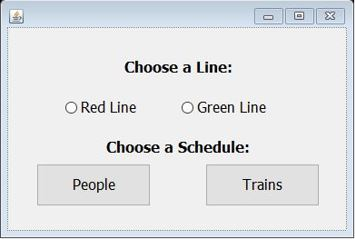
\includegraphics[width=8cm]{main_screen}
	\caption{Start Screen for the MBO and Scheduler.}
\end{figure}


\subsubsection{Choose a Line}
\begin{itemize}
	\item Line Selection Radio-buttons - Clicking on the appropriate radio-button will select which line will be used.
\end{itemize}
\subsubsection{Choose a Schedule}
\begin{itemize}
	\item Click on a button to decide whether you want to view the drivers' or trains' schedule for the line that you selected before.
\end{itemize}

\subsection{Schedule Views}

\begin{figure}[h!]
	\center
	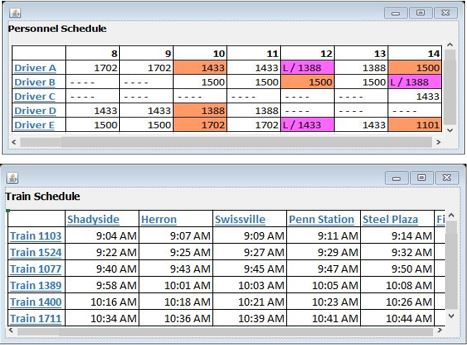
\includegraphics[width=16cm]{schedule_views}
	\caption{Views of the drivers' and trains' schedules.}
\end{figure}

\subsubsection{Personnel Schedule}
\paragraph{Row Headings}
\begin{itemize}
	\item This will display the drivers' names. Clicking on one will display more information about that particular driver.
\end{itemize}
\paragraph{Column Headings}
\begin{itemize}
	\item The time is displayed in the column headings.
\end{itemize}
\paragraph{Table Data}
\begin{itemize}
	\item Inside each cell is the train the driver is operating.
	\item The cells are color coded to display more information.
	\begin{itemize}
		\item Orange means that the driver is scheduled for a break during that time block.
		\item Purple means that the driver is scheduled to take their lunch during that time block.
	\end{itemize}
\end{itemize}

\subsubsection{Train Schedule}
\paragraph{Row Headings}
\begin{itemize}
	\item This will display the trains' IDs. Clicking on one will display more information about that particular train.
\end{itemize}
\paragraph{Column Headings}
\begin{itemize}
	\item This will display the Stations' names. Clicking on one will display more information about that particular station.
\end{itemize}
\paragraph{Table Data}
\begin{itemize}
	\item Inside each cell is the time that the train will arrive at the station.
\end{itemize}

\subsection{Driver View}

\begin{figure}[h!]
	\center
	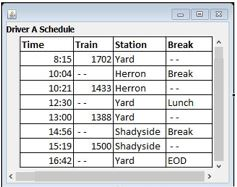
\includegraphics[width=7cm]{driver_view}
	\caption{Views of a particular driver's schedule.}
\end{figure}

\paragraph{Column Headings}
\begin{itemize}
	\item The time, train ID, station, and break status are displayed in the column headings.
\end{itemize}

\subsubsection{Time}
\begin{itemize}
	\item Inside each cell is the time that the driver will arrive at the station.
\end{itemize}

\subsubsection{Train}
\begin{itemize}
	\item Inside each cell is the train that the driver will be operating.
\end{itemize}

\subsubsection{Station}
\begin{itemize}
	\item Inside each cell is the station that the driver will arrive at.
\end{itemize}

\subsubsection{Break}
\begin{itemize}
	\item Inside each cell is the break status of driver during that block.
\end{itemize}


\subsection{Station View}

\begin{figure}[h!]
	\center
	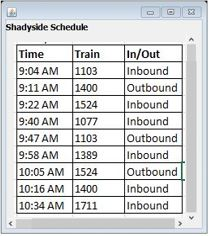
\includegraphics[width=7cm]{station_view}
	\caption{Views of a particular station's schedule.}
\end{figure}

\paragraph{Column Headings}
\begin{itemize}
	\item The time, train ID, Inbound/Outbound status are displayed in the column headings.
\end{itemize}

\subsubsection{Time}
\begin{itemize}
	\item Inside each cell is the time that a train will arrive at the station.
\end{itemize}

\subsubsection{Train}
\begin{itemize}
	\item Inside each cell is the train that will arrive at the station.
\end{itemize}

\subsubsection{Inbound/Outbound}
\begin{itemize}
	\item These cells tell the user whether the train is Inbound to the station or Outbound from the station.
\end{itemize}

\end{document}
